\section{Fase 1. Evaluación del sistema original}
\label{sec:resultados_fase1}

Se identificaron deficiencias mecánicas en los mecanismos de traslación de los ejes X, Y y Z. La configuración inicial incorporó tubos metálicos para instalaciones eléctricas como elementos de guiado y carros impresos en 3D con rodamientos radiales de bolas (Figura~\ref{fig:fase1_vista_general}).

\begin{figure}[H]
    \centering
    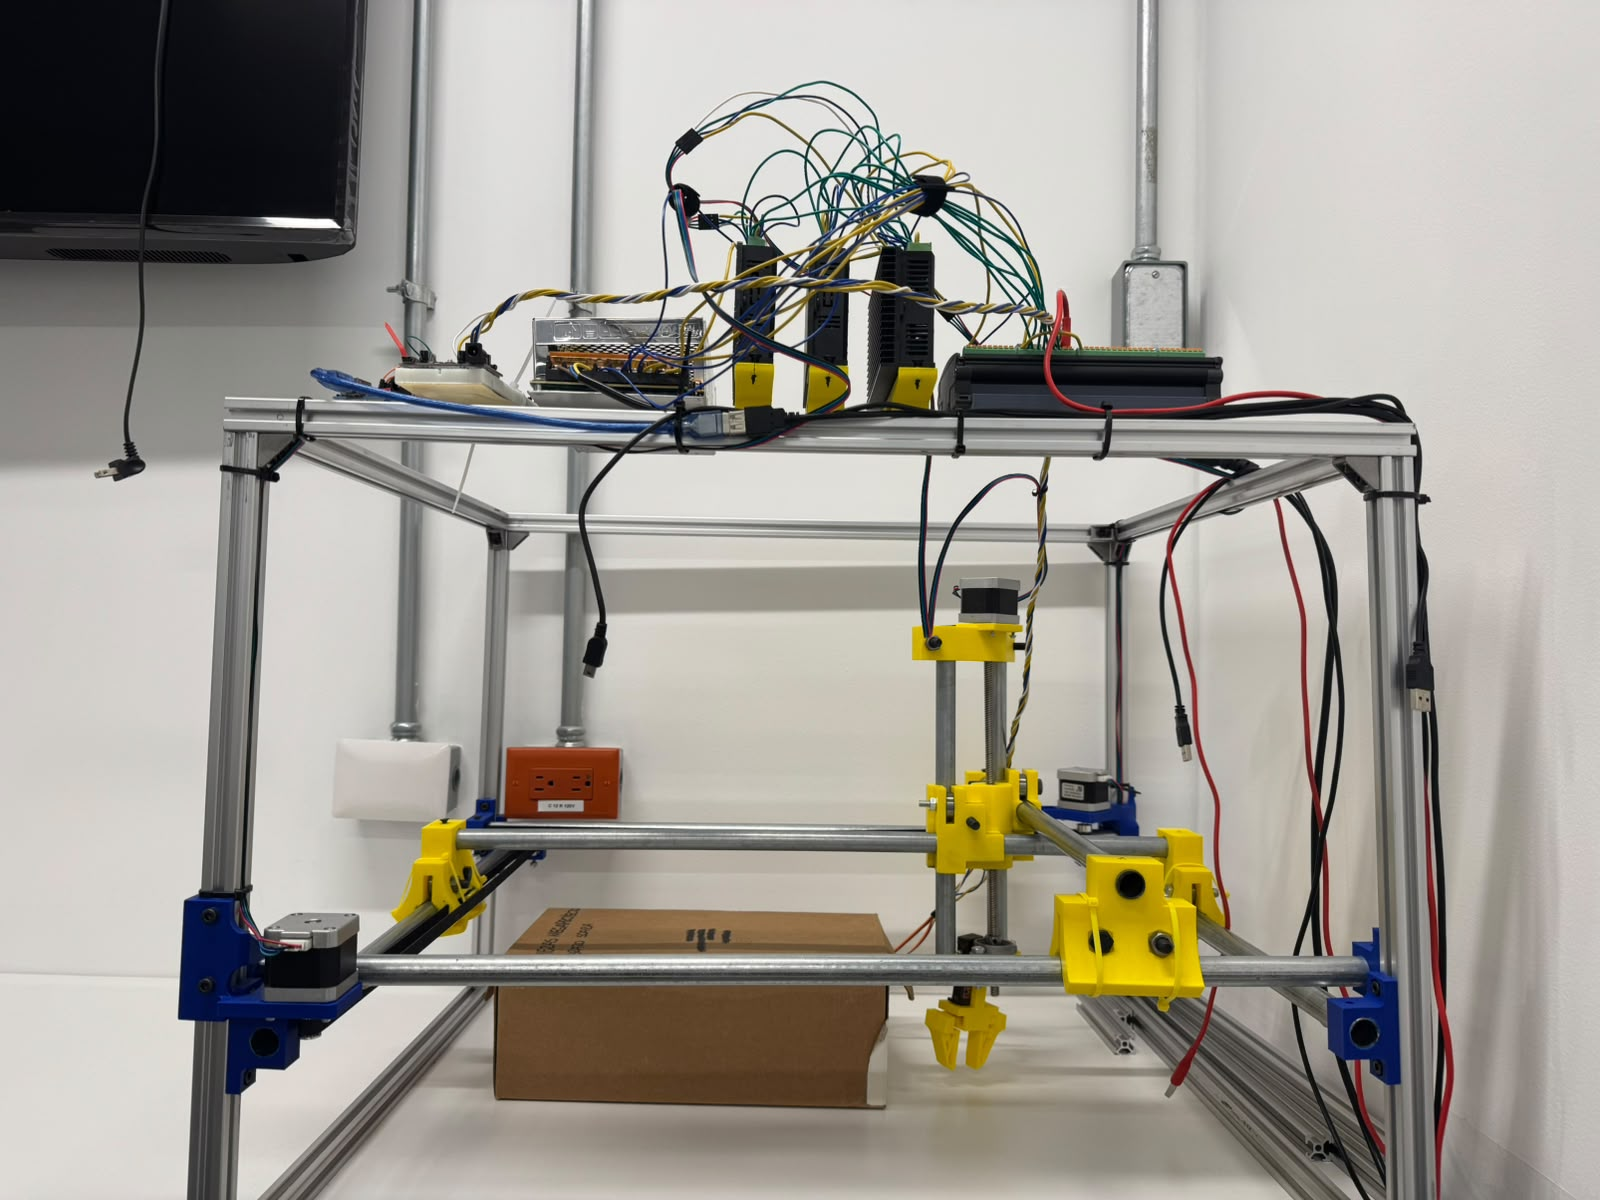
\includegraphics[width=0.75\textwidth,height=6cm,keepaspectratio]{Imagenes de Documentacion/F1_1.jpeg}
    \caption{Configuración inicial del brazo robótico cartesiano.}
    \label{fig:fase1_vista_general}
    \par\small Fuente: elaboración propia.
\end{figure}

En los cuatro carros de X y Y se observó resistencia al desplazamiento y falta de alineación con las guías. También se identificó contacto entre las piezas plásticas y los tubos (Figura~\ref{fig:fase1_carro_xy}). Durante el movimiento del pórtico se observó un avance desigual de sus extremos, identificado como \textit{gantry racking}.

\begin{figure}[H]
    \centering
    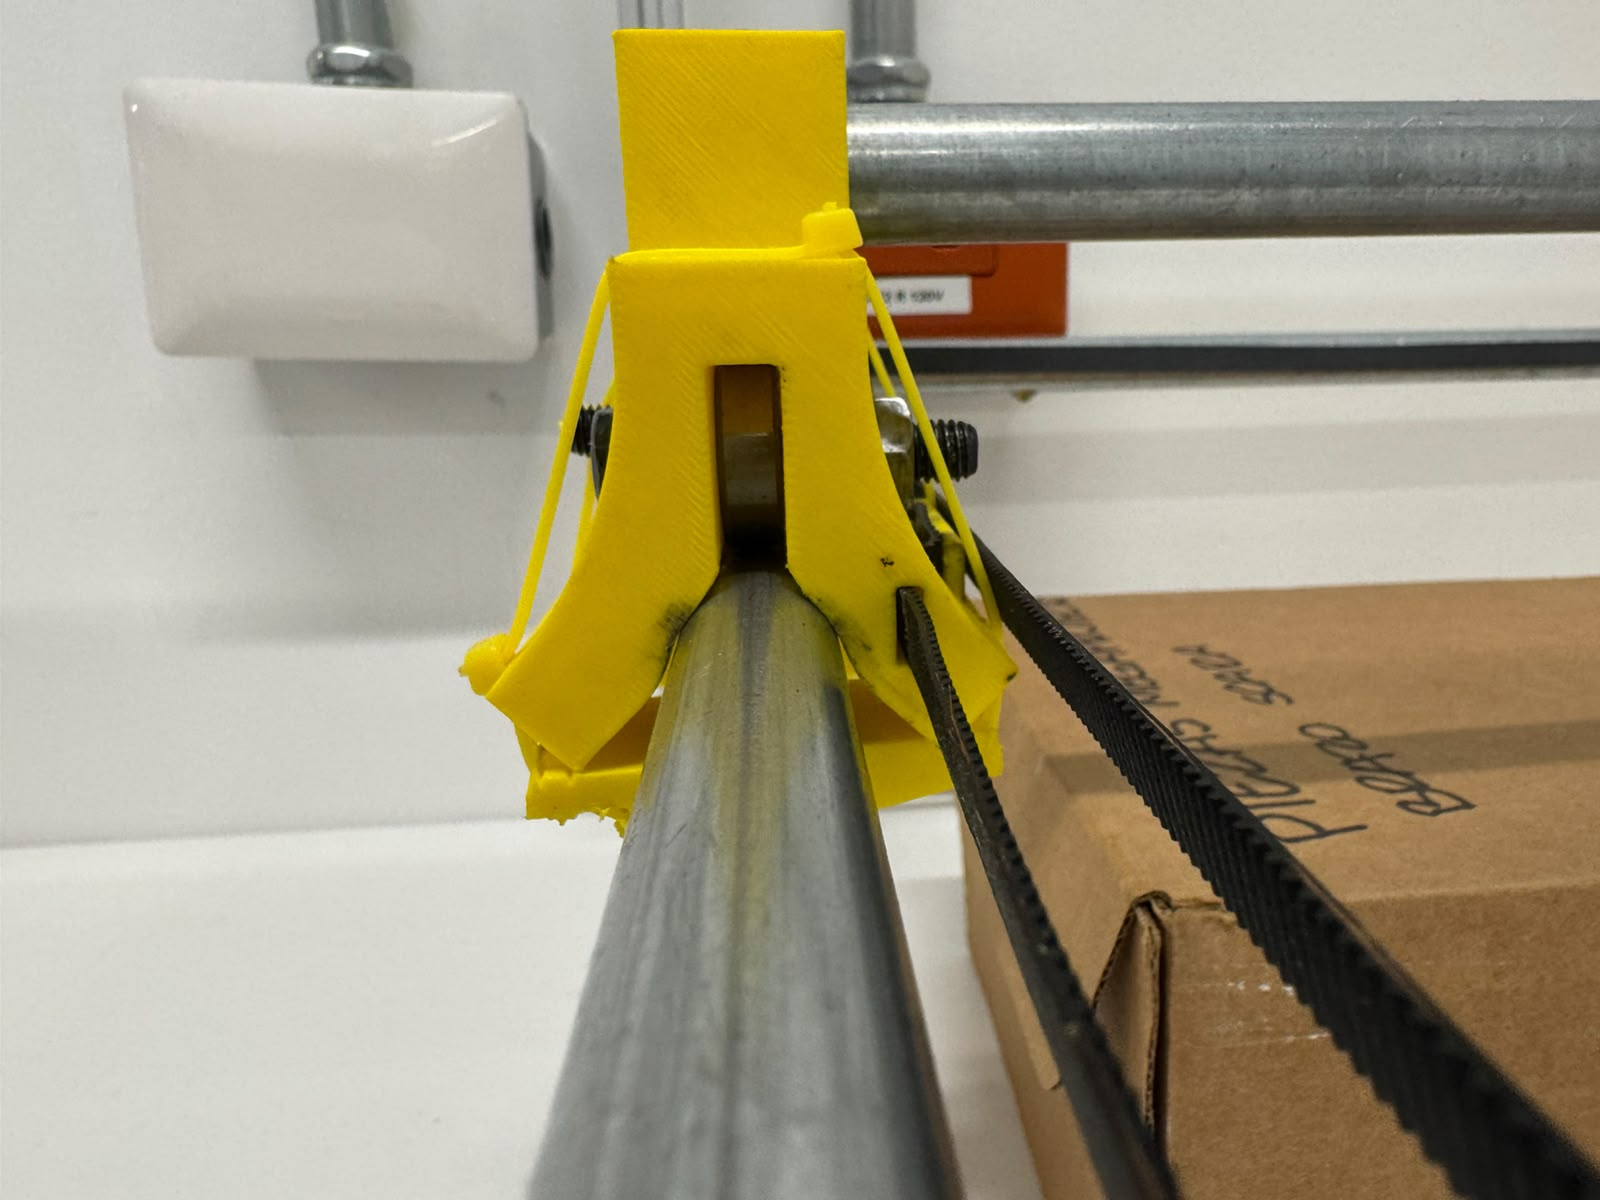
\includegraphics[width=0.65\textwidth,height=5.5cm,keepaspectratio]{Imagenes de Documentacion/F1_3.jpeg}
    \caption{Carro y elementos de guiado del sistema original en X y Y.}
    \label{fig:fase1_carro_xy}
    \par\small Fuente: elaboración propia.
\end{figure}

En Z se observó desalineación del conjunto móvil respecto a la dirección vertical. La disposición del motor, el mecanismo de desplazamiento y la garra se documentó en la Figura~\ref{fig:fase1_eje_z}. Las observaciones de la inspección manual se resumieron en el Cuadro~\ref{tab:fase1_deficiencias}.

\begin{figure}[H]
    \centering
    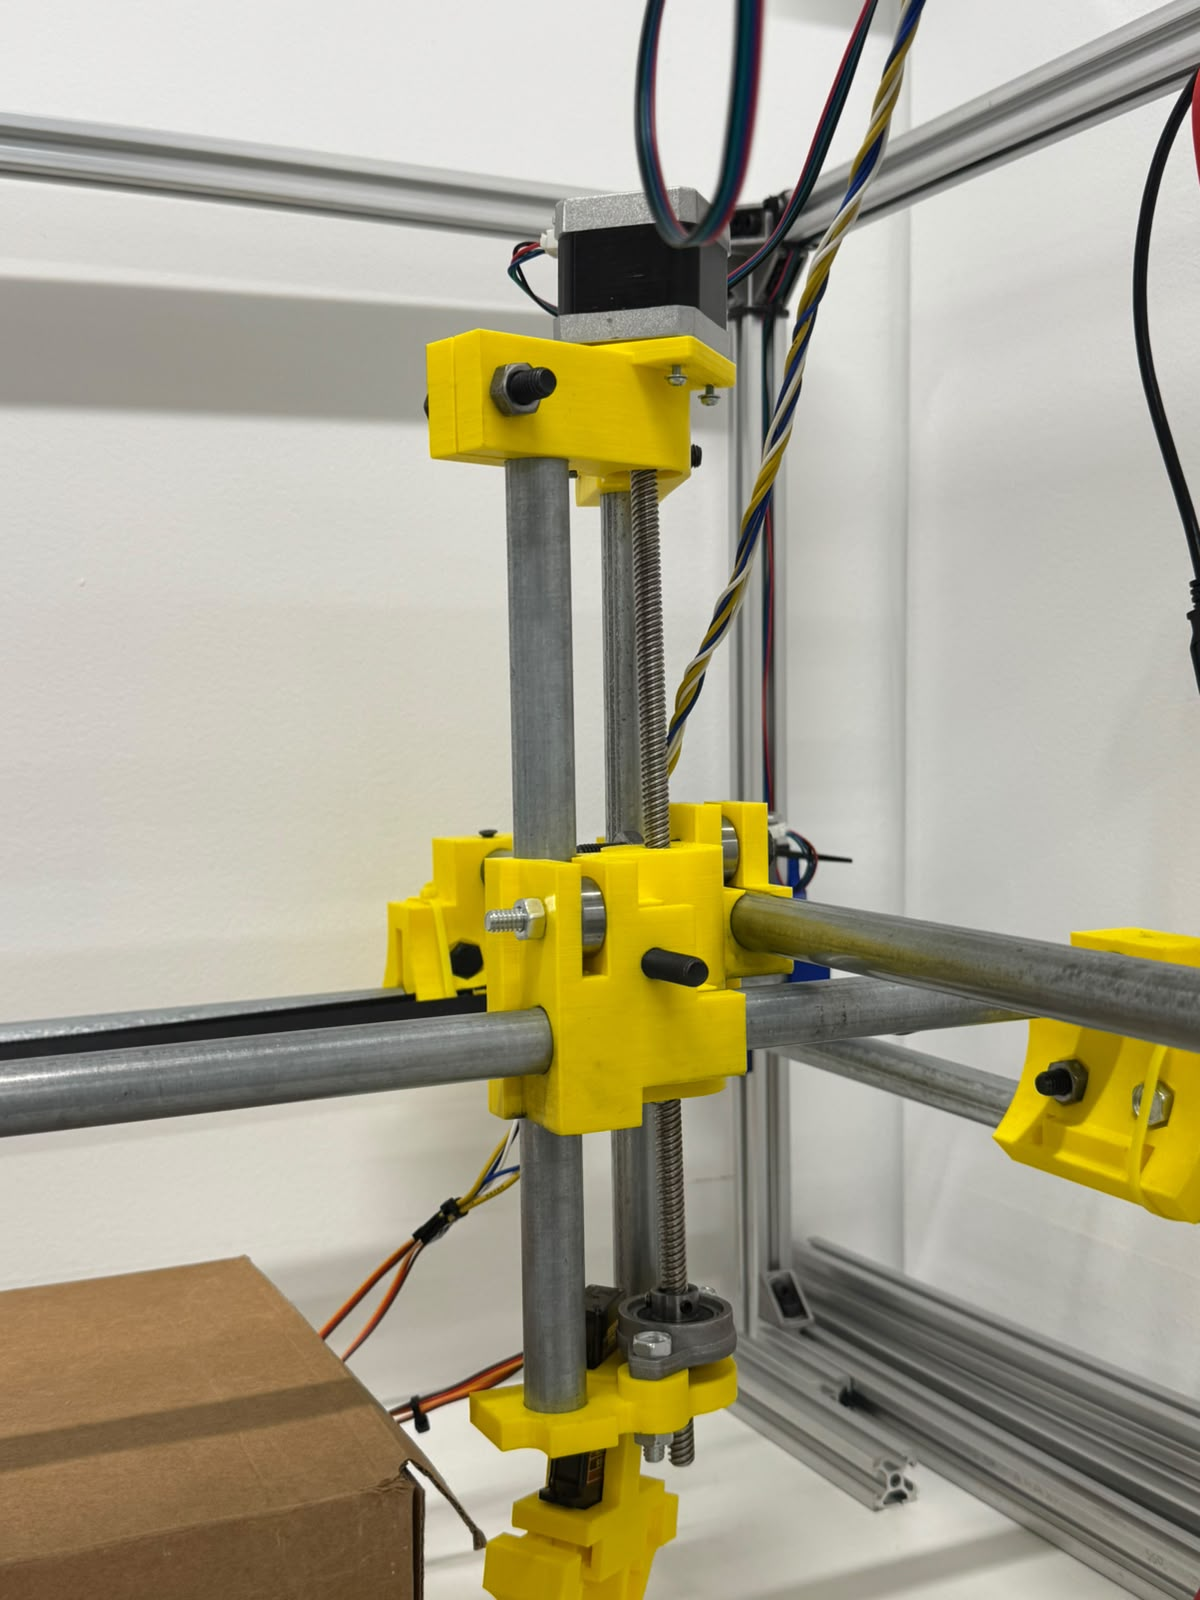
\includegraphics[width=0.55\textwidth,height=5.5cm,keepaspectratio]{Imagenes de Documentacion/F1_4.jpeg}
    \caption{Configuración inicial del mecanismo del eje Z.}
    \label{fig:fase1_eje_z}
    \par\small Fuente: elaboración propia.
\end{figure}

\begin{table}[H]
    \centering
    \caption{Observaciones de la evaluación mecánica inicial.}
    \label{tab:fase1_deficiencias}
    \begin{tabular}{p{0.08\textwidth}p{0.37\textwidth}p{0.43\textwidth}}
        \hline
        Eje & Configuración observada & Hallazgos de la inspección \\
        \hline
        X y Y & Carros impresos con rodamientos radiales sobre tubos metálicos. & Contacto plástico--tubo, resistencia al desplazamiento, desalineación y avance desigual de los extremos del pórtico. \\
        Z & Conjunto vertical con elementos de guiado y soportes impresos. & Desalineación del conjunto móvil y movimiento vertical irregular. \\
        \hline
    \end{tabular}
    \par\small\raggedright Fuente: elaboración propia a partir de la inspección visual y manual.
\end{table}

\section{Fase 2. Selección de componentes y rediseño mecánico}
\label{sec:resultados_fase2}

Se obtuvo un modelo CAD que conservó la arquitectura cartesiana y la disposición general de los ejes X, Y y Z. Se adaptaron los diseños de los soportes de las guías y de los motores de X y Y para incorporar ejes de acero de 12~mm de diámetro. La fabricación de las piezas correspondió a la fase siguiente.

El diseño incluyó cuatro carros para X y Y con rodamientos lineales con carcasa. Cada carro incorporó un paso perpendicular para el eje correspondiente, un espacio para el recorrido de la faja dentada y dos puntos adicionales de fijación (Figura~\ref{fig:fase2_carro_xy}).

\begin{figure}[H]
    \centering
    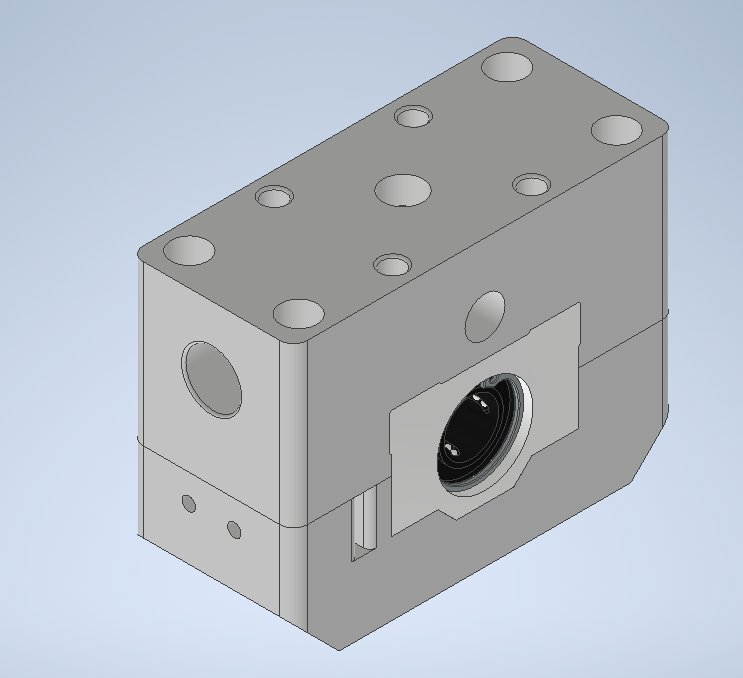
\includegraphics[width=0.65\textwidth,height=5.5cm,keepaspectratio]{Imagenes de Documentacion/F2_1.png}
    \caption{Modelo CAD del carro de traslación de los ejes X y Y.}
    \label{fig:fase2_carro_xy}
    \par\small Fuente: elaboración propia.
\end{figure}

El conjunto central incorporó rodamientos lineales cilíndricos para el desplazamiento en el plano XY. La intersección de ambos ejes quedó ubicada en el centro del conjunto y constituyó la referencia de montaje del mecanismo vertical (Figura~\ref{fig:fase2_centro_xy}).

\begin{figure}[H]
    \centering
    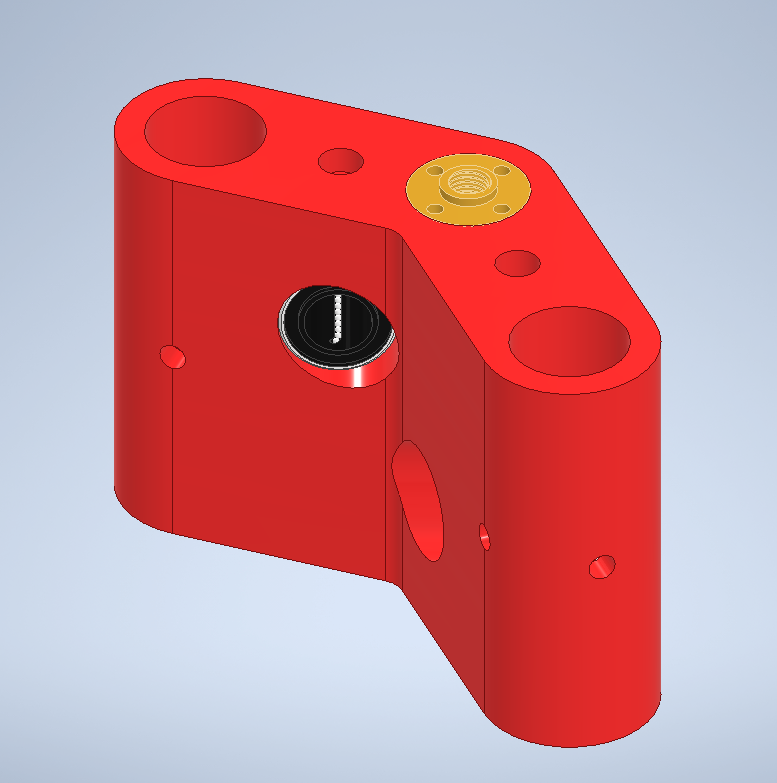
\includegraphics[width=0.65\textwidth,height=5.5cm,keepaspectratio]{Imagenes de Documentacion/F2_2.png}
    \caption{Modelo CAD del conjunto central del mecanismo cartesiano.}
    \label{fig:fase2_centro_xy}
    \par\small Fuente: elaboración propia.
\end{figure}

En el ensamblaje digital, Z incorporó dos guías y un tornillo de avance. Los soportes superior e inferior mantuvieron la separación entre centros definida en el conjunto central (Figura~\ref{fig:fase2_eje_z}). La integración de los componentes se documentó en el ensamblaje general de Autodesk Inventor (Figura~\ref{fig:fase2_ensamble_final}).

\begin{figure}[H]
    \centering
    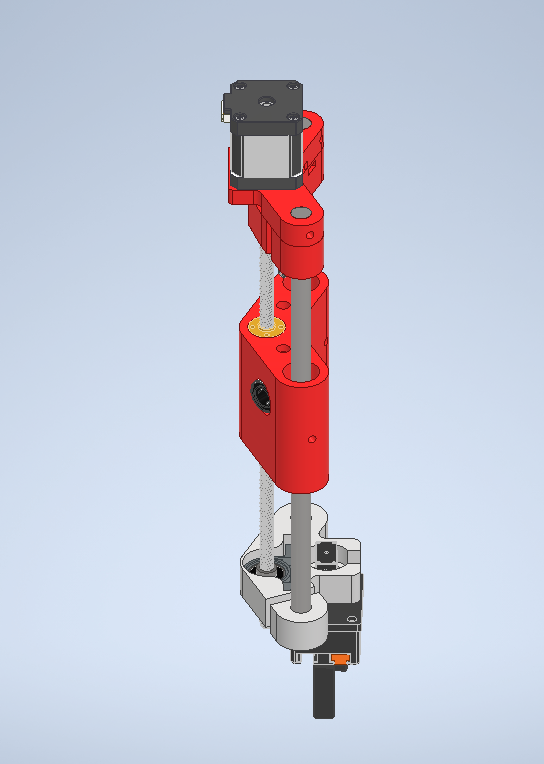
\includegraphics[width=0.60\textwidth,height=6cm,keepaspectratio]{Imagenes de Documentacion/F2_3.png}
    \caption{Modelo CAD del mecanismo vertical integrado al conjunto central.}
    \label{fig:fase2_eje_z}
    \par\small Fuente: elaboración propia.
\end{figure}

\begin{figure}[H]
    \centering
    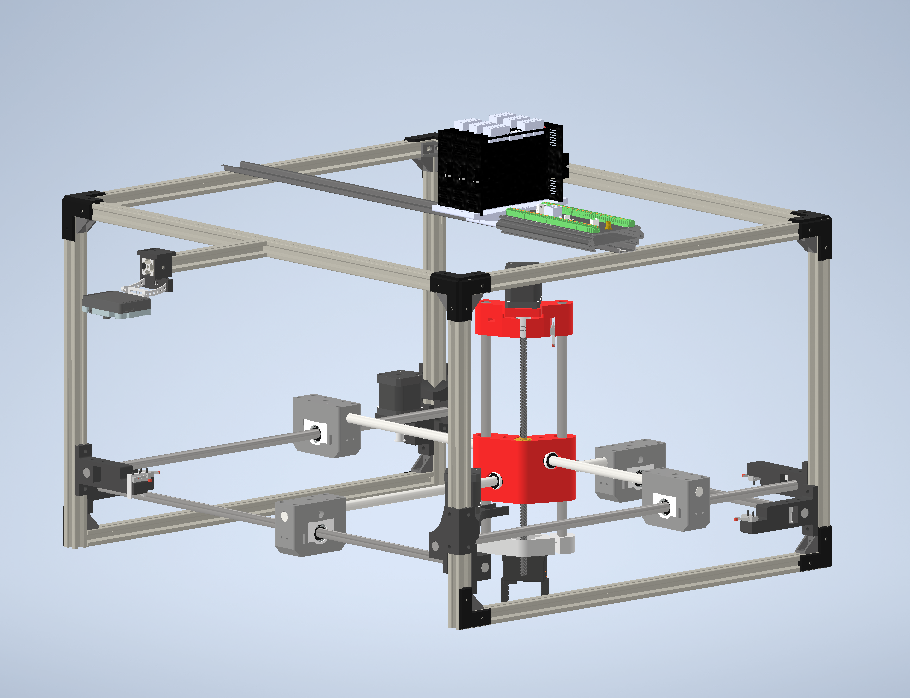
\includegraphics[width=0.75\textwidth,height=6cm,keepaspectratio]{Imagenes de Documentacion/F2_4.png}
    \caption{Ensamblaje CAD del brazo robótico cartesiano en Autodesk Inventor.}
    \label{fig:fase2_ensamble_final}
    \par\small Fuente: elaboración propia.
\end{figure}

% PENDIENTE: confirmar si las imágenes CAD correspondieron a la versión previa
% a fabricar o a una actualización posterior. No se les asignó una iteración.

\section{Fase 3. Implementación mecánica}
\label{sec:resultados_fase3}

\subsection{Componentes fabricados y configuración ensamblada}

Se incorporaron 48 piezas impresas en PLA, incluidas las escuadras de acabado estético. El consumo aproximado de material fue de 1.5~kg, incluidas las pruebas y las iteraciones de fabricación. Todas las piezas impresas se fabricaron nuevamente, incluso aquellas cuyos diseños se retomaron del mecanismo original.

Las piezas obtenidas incluyeron soportes de ejes guía, soportes de montaje de motores, carros de desplazamiento, piezas del conjunto central y soportes de Z. Parte de estos componentes se documentó en la Figura~\ref{fig:fase3_fabricacion}.

\begin{figure}[H]
    \centering
    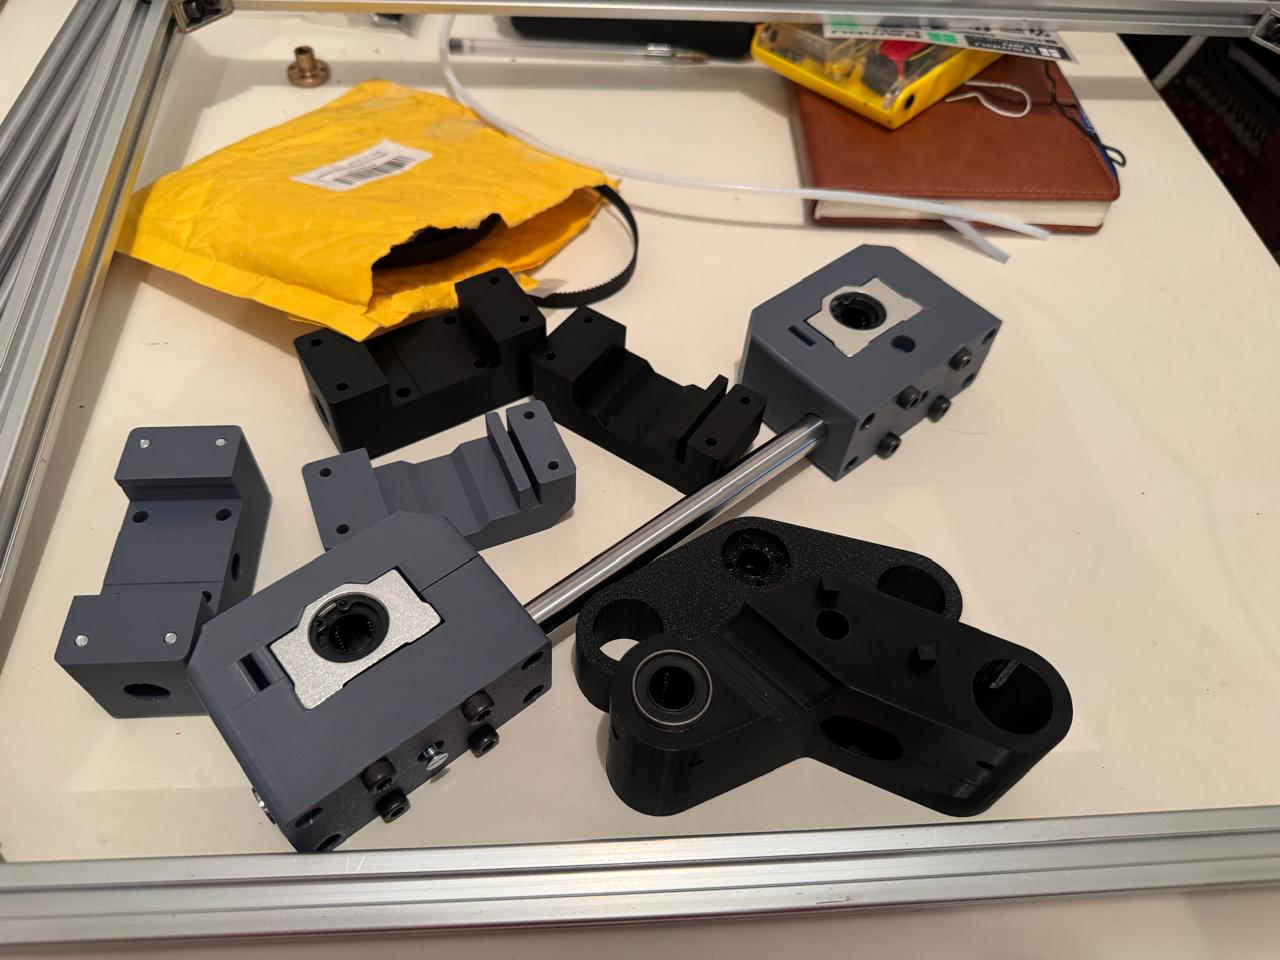
\includegraphics[width=0.72\textwidth,height=6cm,keepaspectratio]{figuras/fase3_componentes.jpeg}
    \caption{Componentes impresos y rodamientos preparados para el ensamblaje.}
    \label{fig:fase3_fabricacion}
    \par\small Fuente: elaboración propia.
\end{figure}

El conjunto ensamblado incorporó perfiles de aluminio 2020 de ranura en T, guías de acero de 12~mm, rodamientos lineales, fajas dentadas para X y Y y un tornillo de avance para Z. Las dimensiones y cantidades reportadas se organizaron en el Cuadro~\ref{tab:fase3_caracteristicas}.

\begin{table}[H]
    \centering
    \caption{Características del conjunto mecánico implementado.}
    \label{tab:fase3_caracteristicas}
    \begin{tabular}{p{0.53\textwidth}p{0.36\textwidth}}
        \hline
        Característica & Valor o configuración \\
        \hline
        Dimensiones generales de la estructura & $700 \times 580 \times 420$~mm \\
        Recorrido reportado del eje X\textsuperscript{a} & 446~mm \\
        Recorrido reportado del eje Y\textsuperscript{a} & 336~mm \\
        Recorrido del eje Z & \textit{Pendiente de medición} \\
        Diámetro de los ejes guía & 12~mm \\
        Ejes de 700~mm & 3 unidades \\
        Ejes de 580~mm & 3 unidades \\
        Perfiles estructurales & Aluminio 2020 de ranura en T \\
        Piezas impresas incorporadas & 48 unidades \\
        Material de las piezas impresas & PLA \\
        Consumo aproximado de PLA, incluidas las pruebas & 1.5~kg \\
        Transmisión en X y Y & Fajas dentadas \\
        Transmisión en Z & Tornillo de avance \\
        \hline
    \end{tabular}
    \par\small\raggedright Fuente: elaboración propia a partir de los datos de fabricación y ensamblaje del proyecto.
    \par\small La altura se refirió a la superficie de la mesa. El consumo de PLA incluyó las pruebas y no correspondió a la masa del brazo ensamblado.
    \par\small\textsuperscript{a} Se conservaron los valores reportados; su procedencia, del modelo CAD o de medición física, quedó pendiente de confirmación.
\end{table}

\subsection{Configuraciones del conjunto central y del soporte de la garra}

El conjunto central pasó por tres iteraciones. En las dos primeras se presentaron dificultades de retención de los rodamientos; en la configuración final estos permanecieron en sus alojamientos durante las comprobaciones de movimiento. Las configuraciones y sus observaciones se resumieron en el Cuadro~\ref{tab:fase3_iteraciones}.

\begin{table}[H]
    \centering
    \caption{Iteraciones del conjunto central y observaciones de montaje.}
    \label{tab:fase3_iteraciones}
    \begin{tabular}{p{0.10\textwidth}p{0.38\textwidth}p{0.40\textwidth}}
        \hline
        Iteración & Configuración & Observación \\
        \hline
        Primera & Cuerpo inicial al que se añadieron tornillos de presión. & Se observó la salida de los rodamientos de sus alojamientos antes de incorporar los tornillos. \\
        Segunda & Conjunto dividido en tres piezas con tornillos de presión. & Persistieron las dificultades de sujeción de los rodamientos. \\
        Tercera & Conjunto con tornillos de unión entre las piezas. & Los rodamientos permanecieron en sus alojamientos durante las comprobaciones realizadas. \\
        \hline
    \end{tabular}
    \par\small\raggedright Fuente: elaboración propia a partir de la descripción del proceso de fabricación y ensamblaje.
\end{table}

El conjunto central ensamblado y una vista del montaje parcial se documentaron en la Figura~\ref{fig:fase3_montaje}. El soporte inferior de Z incorporó una unión desmontable para la garra, en sustitución de la unión fija inicial. El efector final quedó ubicado en la intersección de los ejes del conjunto central.

\begin{figure}[H]
    \centering
    \begin{minipage}[b]{0.38\textwidth}
        \centering
        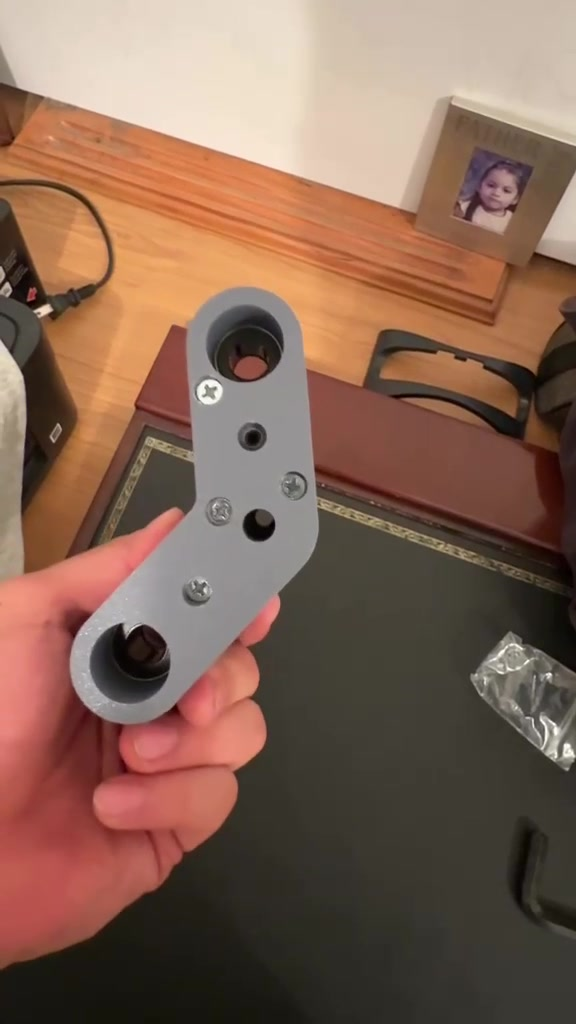
\includegraphics[width=\linewidth,height=6.5cm,keepaspectratio]{figuras/fase3_central_inferior.jpg}
        \par\small (a) Conjunto central ensamblado.
    \end{minipage}
    \hfill
    \begin{minipage}[b]{0.58\textwidth}
        \centering
        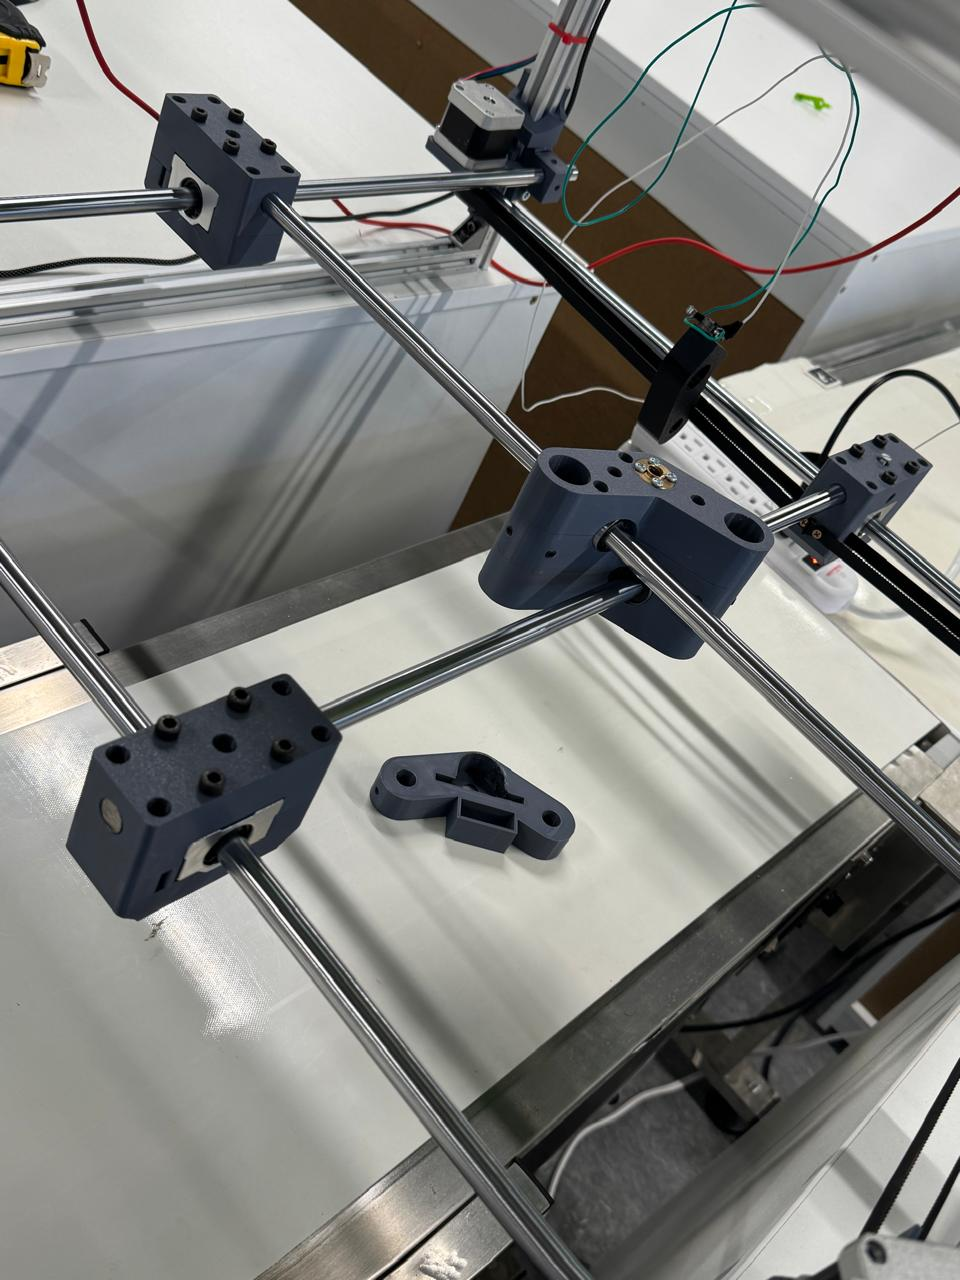
\includegraphics[width=\linewidth,height=6.5cm,keepaspectratio]{figuras/fase3_ensamblaje_parcial.jpeg}
        \par\small (b) Montaje parcial de guías y carros.
    \end{minipage}
    \caption{Conjunto central y montaje parcial del mecanismo cartesiano.}
    \label{fig:fase3_montaje}
    \par\small Fuente: elaboración propia; fotografía y fotograma del registro audiovisual del proyecto.
\end{figure}

\subsection{Comprobación mecánica preliminar}

Se comprobó el desplazamiento de los tres ejes mediante manipulación directa, antes del accionamiento electrónico. Los carros permanecieron sobre sus guías y no se reprodujeron los atascos identificados en el mecanismo original durante las comprobaciones realizadas.

La resistencia al movimiento se percibió menor que en el sistema original. El avance desigual de los extremos del pórtico resultó poco perceptible durante la inspección visual. Se observaron vibraciones leves y no se identificó deflexión de las guías a simple vista. Estas observaciones fueron cualitativas y no correspondieron a mediciones de precisión o repetibilidad.

\section{Fase 4. Accionamiento electrónico, operación manual y referenciación}
\label{sec:resultados_fase4}

\subsection{Distribución de funciones e interfaces}

El circuito de prueba se montó en protoboards y se emplearon conductores calibre AWG~22 en las interconexiones entre módulos y microcontroladores, según el registro de montaje del autor. En las fotografías se documentaron las placas de conexiones, las borneras y un controlador de motor paso a paso identificado como DM542T (Figura~\ref{fig:fase4_montaje}). Las imágenes no permitieron determinar las tensiones de alimentación ni los ajustes de corriente y micropasos del controlador.

\begin{figure}[H]
    \centering
    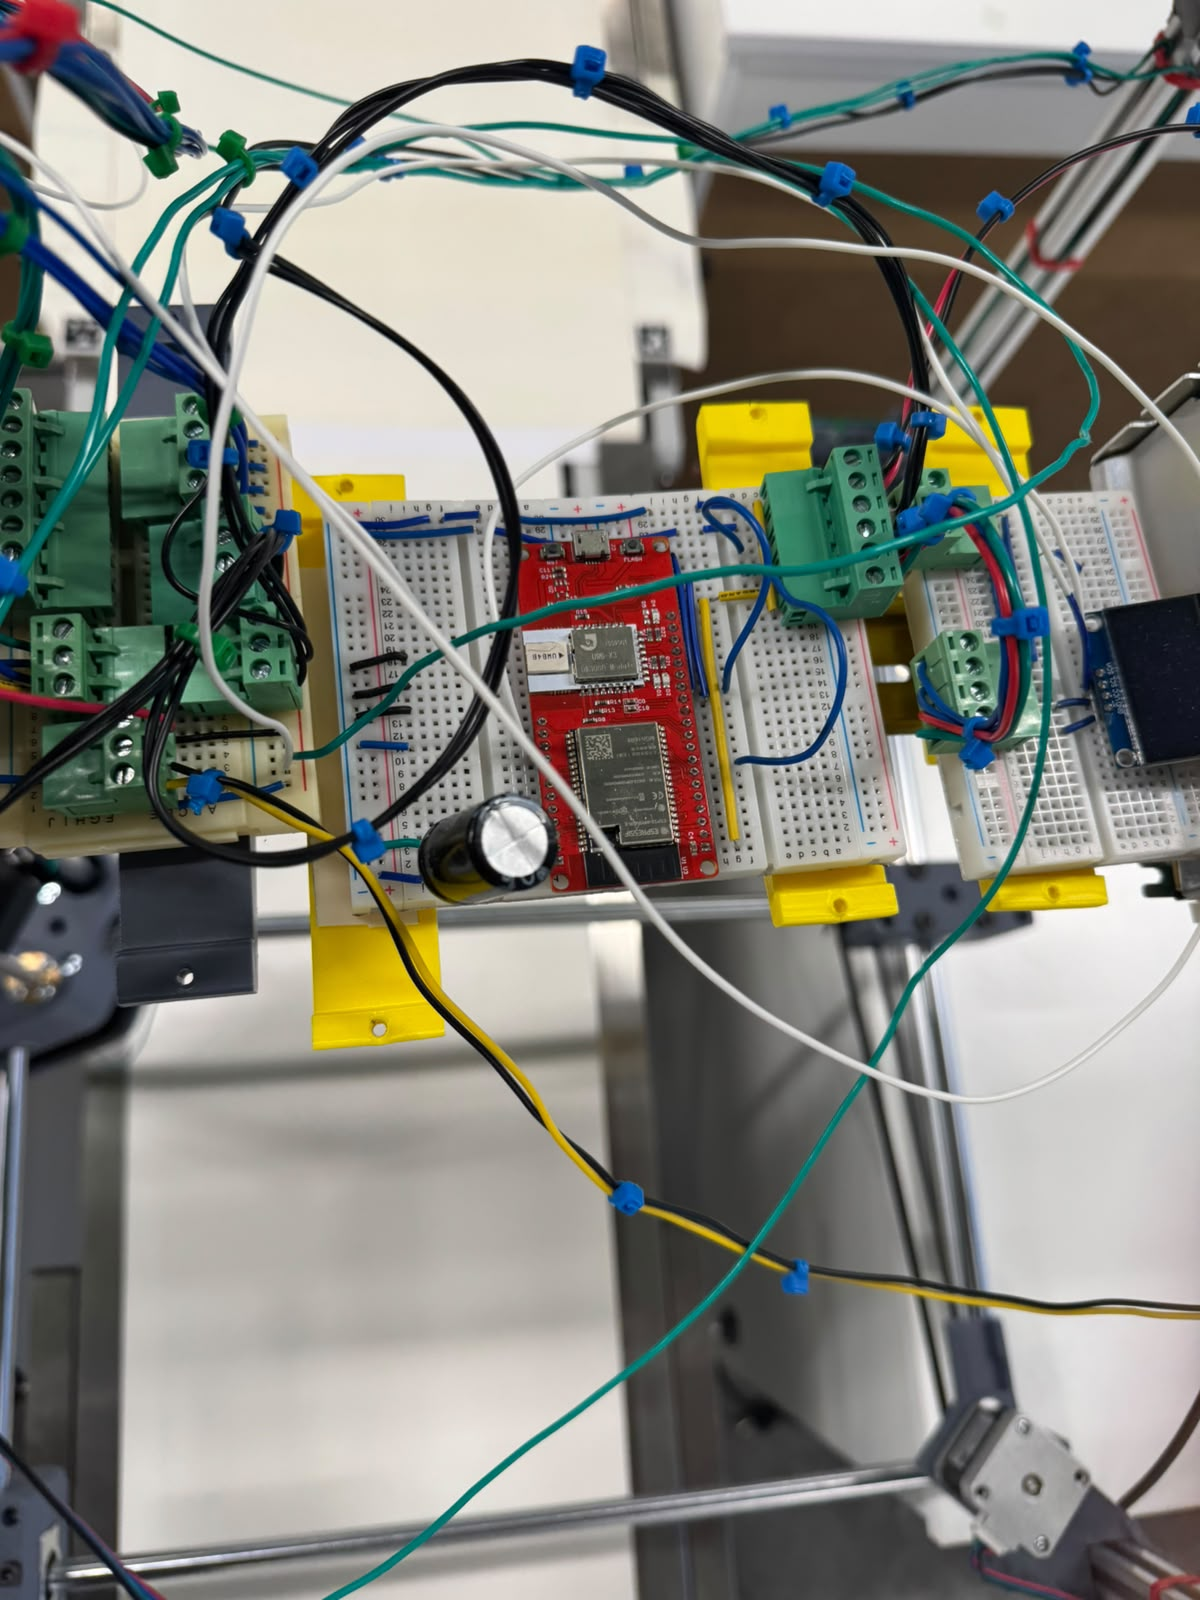
\includegraphics[width=0.42\textwidth]{figuras_fase4/montaje_protoboard.png}\hfill
    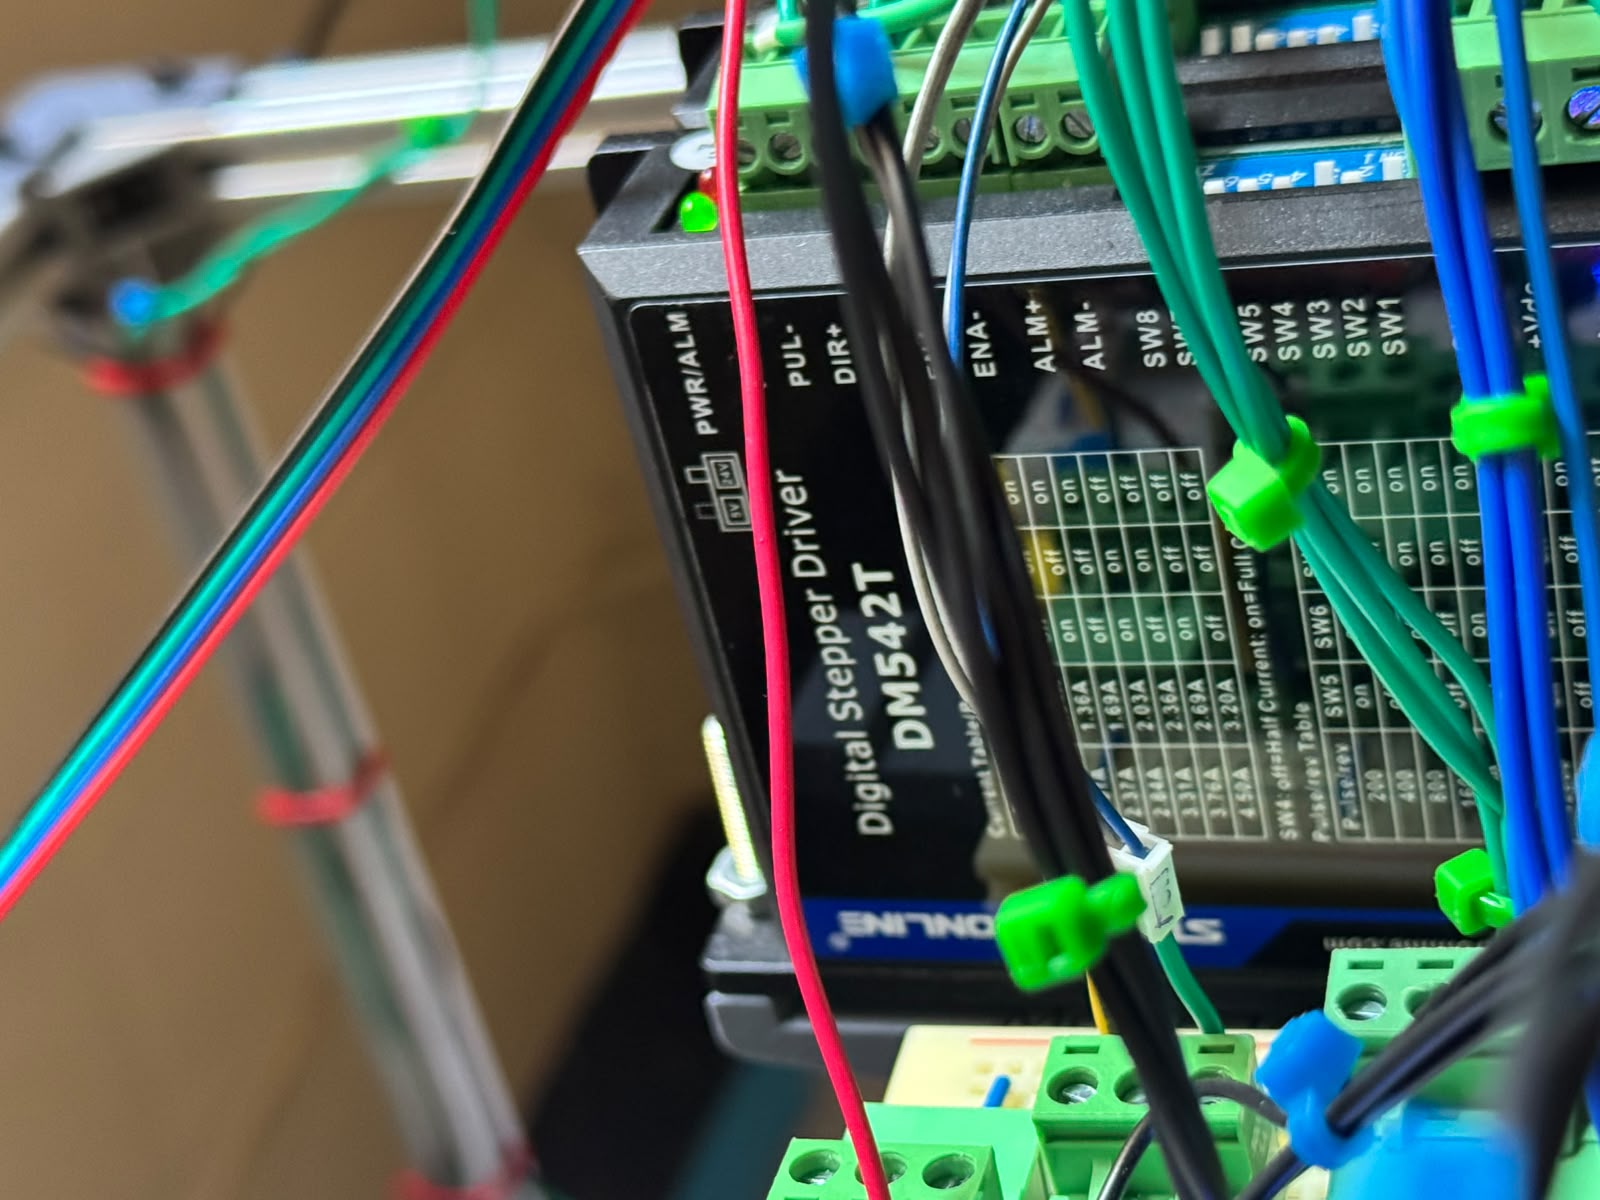
\includegraphics[width=0.53\textwidth]{figuras_fase4/driver_dm542t.png}
    \caption{Montaje electrónico en protoboards (izquierda) e identificación del controlador DM542T (derecha).}
    \label{fig:fase4_montaje}
    \par\small\raggedright Fuente: registro fotográfico del autor.
\end{figure}

Se obtuvo una implementación distribuida entre la ESP32 y la Portenta H7 con Machine Control. La ESP32 recibió las entradas del mando, accionó los servomotores y presentó la información en la OLED. La Portenta generó las señales de los motores paso a paso, adquirió los finales de carrera y ejecutó la calibración y la máquina de estados del sistema.

La comunicación entre placas se configuró mediante I2C a 100~kHz, con la Portenta como maestra y la ESP32 como esclava en la dirección \texttt{0x40}. La pantalla utilizó otro bus I2C de la ESP32, independiente del enlace entre placas. Las asignaciones del firmware se resumieron en el Cuadro~\ref{tab:fase4_interfaces}.

\begin{table}[H]
    \centering
    \caption{Interfaces y asignaciones del firmware revisado.}
    \label{tab:fase4_interfaces}
    \begin{tabular}{p{0.24\textwidth}p{0.64\textwidth}}
        \hline
        Elemento & Configuración \\
        \hline
        Enlace entre placas & I2C, 100~kHz; ESP32: SDA en GPIO27 y SCL en GPIO14, dirección \texttt{0x40}. \\
        OLED & Controlador SH1106, $128\times64$ píxeles; SDA en GPIO21, SCL en GPIO22, dirección \texttt{0x3C}, 100~kHz. \\
        Servomotores & Señales de rotación y pinza en GPIO25 y GPIO26 de la ESP32, respectivamente; frecuencia configurada a 50~Hz. \\
        Movimiento X & Canales de salida 4 para STEP y 5 para DIR de Machine Control. \\
        Movimiento Y & Canales de salida 2 para STEP y 3 para DIR de Machine Control. \\
        Movimiento Z & Canales de salida 0 para STEP y 1 para DIR de Machine Control. \\
        Finales de carrera & DIN00: X mínimo; DIN01: X máximo; DIN02: Y mínimo; DIN03: Y máximo; DIN04: Z abajo; DIN05: Z arriba. \\
        \hline
    \end{tabular}
    \par\small\raggedright Fuente: elaboración propia a partir de los archivos ESP.ino y PORTENTA.ino de la carpeta de pruebas.
    \par\small Las asignaciones correspondieron al firmware; los canales de Machine Control no equivalieron a números GPIO de la ESP32.
\end{table}

\subsection{Comunicación I2C entre los microcontroladores}

El enlace I2C utilizó las líneas SDA y SCL, asignadas a GPIO27 y GPIO14 de la ESP32. La Portenta inició las transacciones de lectura y escritura a la dirección \texttt{0x40}; la ESP32 respondió como dispositivo esclavo. La generación de órdenes del mando en la ESP32 no modificó estos papeles del bus. En paralelo, la ESP32 gestionó la OLED en un segundo bus, mediante GPIO21 y GPIO22 y la dirección \texttt{0x3C}.

Sobre el enlace entre placas se implementó un formato binario propio, identificado en el código como versión 5. Esta numeración correspondió al formato de los mensajes de la aplicación, no a una versión del estándar I2C. Se definieron dos estructuras de 32 bytes, una para cada sentido del intercambio, y se verificó su tamaño mediante comprobaciones de compilación. Ambas incluyeron identificación, versión y longitud en sus tres primeros bytes y un CRC-8/ATM en el último. El CRC se calculó sobre los 31 bytes precedentes, con valor inicial \texttt{0x00} y polinomio \texttt{0x07}.

Los campos vinculados con la operación manual se resumieron en el Cuadro~\ref{tab:fase4_paquetes}. La versión integrada también incluyó campos de visión y funcionamiento automático, cuyo análisis se reservó para la fase posterior; estos campos se conservaron dentro de los tamaños indicados.

\begin{table}[H]
    \centering
    \caption{Distribución de los paquetes I2C en la versión de software revisada.}
    \label{tab:fase4_paquetes}
    \begin{tabular}{p{0.22\textwidth}p{0.55\textwidth}r}
        \hline
        Sentido & Campos agrupados & Bytes \\
        \hline
        ESP32 a Portenta & Identificación, versión y longitud & 3 \\
        & Secuencia de paquete y sesión de arranque & 3 \\
        & Indicadores, direcciones X/Y/Z, botones y ángulos ordenados a los servos & 7 \\
        & Campos adicionales de la versión integrada & 18 \\
        & CRC & 1 \\
        \hline
        Portenta a ESP32 & Identificación, versión y longitud & 3 \\
        & Estado, opción de menú, fase de calibración, indicadores del sistema, límites, movimientos y error & 7 \\
        & Campos adicionales de la versión integrada & 21 \\
        & CRC & 1 \\
        \hline
    \end{tabular}
    \par\small\raggedright Fuente: elaboración propia a partir de las estructuras de ProtocoloI2C.h.
\end{table}

La ESP32 preparó una copia de sus datos mediante \texttt{prepararSnapshotI2C()}, con un intervalo programado de 10~ms. Cuando la Portenta solicitó una lectura mediante \texttt{Wire.requestFrom()}, la función \texttt{requestEvent()} entregó esa copia. La Portenta comprobó el número de bytes, la identificación, la versión, la longitud declarada, el CRC y la validez de los valores recibidos antes de actualizar las órdenes. En modo manual, \texttt{procesarModoManual()} utilizó las direcciones admitidas para ejecutar el movimiento de los ejes. Los servomotores permanecieron bajo accionamiento local de la ESP32; sus ángulos incluidos en el paquete correspondieron a consignas, no a mediciones.

En el sentido contrario, \texttt{enviarPaquetePortenta()} inició una escritura con el estado del sistema, la fase de calibración, los límites y los movimientos. En la ESP32, \texttt{receiveEvent()} almacenó el mensaje recibido y \texttt{procesarRecepcionI2C()} efectuó su validación fuera de esa función de recepción. La información aceptada actualizó el estado remoto utilizado por la interfaz. Así, el flujo de operación quedó constituido por la lectura del mando en la ESP32, el sondeo desde la Portenta, la ejecución de órdenes y el envío del estado hacia la ESP32.

En la Portenta se programaron intervalos de 10~ms para el sondeo del control y de 20~ms para el envío de estados. Cuando ambas operaciones quedaron pendientes en la misma iteración, se priorizó el envío de estados y la lectura se atendió en una iteración posterior. Estos intervalos correspondieron a la planificación del programa y no a mediciones de latencia ni a una garantía de periodicidad exacta.

La supervisión del enlace incluyó la antigüedad del último paquete válido y del último cambio de su número de secuencia, con umbrales de 150~ms en la Portenta. También se incorporaron la detección de cambios de sesión de arranque de la ESP32 y un umbral de diez paquetes inválidos consecutivos. Fuera de los estados iniciales de espera, las condiciones de fallo contempladas condujeron a la detención y al estado de error. En la ESP32, el estado recibido de la Portenta se invalidó cuando su antigüedad superó 1000~ms. Se mantuvieron contadores de lecturas, escrituras y errores para el diagnóstico por terminal; no se atribuyeron tasas de error medidas a esos contadores sin registros de ensayo.

\subsection{Movimiento manual e interfaz de usuario}

Las entradas horizontales y verticales del joystick izquierdo se asignaron a X y Y. La entrada vertical del joystick derecho se asignó a Z y la horizontal al servo de rotación. La cruceta modificó el ángulo de la pinza. Para los ejes se utilizó un umbral de zona neutra de 100 unidades de lectura y se generaron órdenes discretas de dirección $-1$, $0$ y $1$.

La Portenta ejecutó el desplazamiento continuo solicitado mientras la orden permaneció activa y el final correspondiente no bloqueó ese sentido. La implementación incluyó detención al neutralizar el mando, al abandonar el modo manual o al detectar la desconexión del control. También incorporó comprobaciones de vigencia de los paquetes y de activación simultánea de los dos finales de un mismo eje.

En modo manual, la OLED presentó las direcciones de movimiento de X, Y y Z, los estados de los límites de X y Y y los ángulos ordenados a los dos servos. Durante la calibración mostró la fase y el campo de estados de los límites. La pantalla manual no presentó una medición de posición cartesiana ni los dos límites de Z como indicadores individuales.

Las principales funciones implementadas se organizaron en el Cuadro~\ref{tab:fase4_funciones}. Su identificación documentó la estructura del software y no constituyó una medición de desempeño físico.

\begin{table}[H]
    \centering
    \caption{Funciones principales del accionamiento y de la operación manual.}
    \label{tab:fase4_funciones}
    \begin{tabular}{p{0.45\textwidth}p{0.43\textwidth}}
        \hline
        Función o grupo & Función implementada \\
        \hline
        \texttt{generarPulsoMotor()} & Generación de STEP y actualización del conteo de pasos de cada eje. \\
        \texttt{moverXContinuo()}, \texttt{moverYContinuo()}, \texttt{moverZContinuo()} & Accionamiento por dirección sin destino de pasos prefijado. \\
        \texttt{leerFinalesCarrera()}, \texttt{aplicarBloqueoPorFinales()} & Adquisición de límites y detención del movimiento hacia el límite activo. \\
        \texttt{processControllers()} & Lectura del mando y actualización de las órdenes de movimiento y servos en la ESP32. \\
        \texttt{prepararSnapshotI2C()}, \texttt{leerPaqueteESP32()} & Preparación de datos en la ESP32 y lectura y validación desde la Portenta. \\
        \texttt{procesarModoManual()} & Ejecución de las órdenes direccionales admitidas en la Portenta. \\
        \texttt{procesarCalibracionBrazo()} & Recorrido de los límites y establecimiento de la referencia de los tres ejes. \\
        \texttt{mostrarModoManual()} & Presentación de las variables del modo manual en la OLED. \\
        \hline
    \end{tabular}
    \par\small\raggedright Fuente: elaboración propia a partir del código de pruebas.
\end{table}

\subsection{Referenciación y posicionamiento cartesiano}

La rutina de calibración recorrió sucesivamente X, Y y Z. En cada extremo se programaron una primera aproximación, la liberación del sensor, una separación adicional de 300 pasos y una segunda aproximación más lenta. Se rechazaron los rangos inferiores a 100 pasos y se estableció un límite de 180~s por fase. Estos valores correspondieron a parámetros programados, no a tiempos o recorridos medidos durante un ensayo.

El procedimiento determinó el recorrido de cada eje en pasos y ordenó el desplazamiento a su punto medio. Al completar ese movimiento, los contadores de X, Y y Z se reiniciaron a cero. Por tanto, el origen definido por la calibración correspondió al centro del recorrido contado y no a uno de los extremos.

Para X y Y se implementaron los factores de conversión de la Ecuación~\ref{eq:fase4_escala}. Los valores $N_X$ y $N_Y$ correspondieron a los conteos entre extremos; $L_X$ y $L_Y$ correspondieron a las longitudes configuradas en el firmware.

\begin{equation}
    s_X=\frac{N_X}{L_X},\qquad s_Y=\frac{N_Y}{L_Y},\qquad
    n_X=\operatorname{round}(x\,s_X),\qquad
    n_Y=\operatorname{round}(y\,s_Y).
    \label{eq:fase4_escala}
\end{equation}

El código utilizó $L_X=446$~mm y $L_Y=336$~mm. El recorrido físico de Y se estableció en 336~mm, según la confirmación del autor, y coincidió con el valor configurado para calcular su escala.

La función \texttt{cinematicaInversaCartesiana()} convirtió las coordenadas X/Y en destinos de pasos y comprobó un margen de 2~mm respecto de los extremos. El comando \texttt{GOTO X Y Z} admitió tres argumentos, pero \texttt{iniciarMovimientoXY()} ejecutó únicamente los destinos de X y Y. El argumento Z se recibió sin ordenar un desplazamiento de ese eje. El comando de terminal \texttt{HOME} también actuó únicamente sobre X/Y, a diferencia de la rutina de calibración inicial de los tres ejes.

El posicionamiento por coordenadas y el desplazamiento direccional por joystick quedaron implementados como rutas distintas. En la versión revisada, \texttt{procesarModoManual()} no invocó la función de cinemática inversa.
